\documentclass[../main/main.tex]{subfiles}

\begin{document}

\newpage
\chapter{Evaluation}
\section{Objectives}
\subsection{Objective 1}
All laser chess game logic should be properly implemented. Refer to Figure \ref{fig:evaluation-game}.

Both the play and review screens display a 10x8 laser chess board. Players can move and rotate pieces on their respective turns, with the laser firing and destroying pieces automatically. The game ends when a player draws, resigns, has their pharoah destroyed or reaches three-fold repetition.

Objective 1 is fulfilled, the game plays successfully. A possible improvement would be an option to play against local hosts. This was not a requested or planned feature, but would be very handy for a two-player game.

\subsection{Objective 2}
Save or load game options should be implemented. Refer to Figures \ref{fig:evaluation-browser} and \ref{fig:evaluation-review}.

In the browser screen, users can scroll through all previous games, with the option to delete or review them, or copy their FEN string. Games can be sorted, and pages of games can be scrolled through. The game positions are encoded using a custom FEN string format, and games are saved as rows in a local SQLite database table. In the review screen, users can scroll through all the moves of a previous game. The right side bar displays information such as the winner and move number, and the timer, pieces and move list updates accordingly.

Objective 2 is fulfilled. A possible improvement would be to add the option of loading up a position to resume playing straight from the review screen. This would be a convenient feature, but is not a priority, as users can currently copy the FEN string from the browser screen to the config screen and load the position there as an alternative option.

\subsection{Objective 3}
Other board game requirements should be implemented. Refer to Figure \ref{fig:evaluation-game}.

In addition to the core game mechanics, other ancilliary aspects are added as well. The piece display correctly updates to show all destroyed pieces. Timers can be enabled and disabled, decrement correctly, and end the game when they run out. Buttons also exist for drawing and resigning the game. The move list and status message widgets also provide update accordingly and provide information on the stage of the game.

Objective 3 is fulfilled.

\subsection{Objective 4}
Game settings and config should be customisable. Refer to Figures \ref{fig:evaluation-settings} and \ref{fig:evaluation-config} and \ref{fig:evaluation-editor}.

In the settings screen, the user can change settings to toggle the volume, fullscreen, board colours, particles and shaders. All settings update correctly, and are saved to a local JSON file when the settings screen is exited. The game configurations are changed in the config screen. Here, users can change the game's starting colour, configure timer settings, change to the CPU player and specify the difficulty, select a board preset, or create a custom board layout through the editor screen. The editor screen comes with all the basic operations of placing pieces, rotating pieces, and erasing and dragging them.

Objective 4 is fulfilled.

\subsection{Objective 5}
Game UI should improve player experience. Refer to Figure \ref{fig:evaluation-game}.

When a player holds down on a piece, the piece can be moved through drag-and-drop. Indicators are also present to show adjacent squares that the piece can be moved to. Audio cues also improve the immersiveness of the game, as well as the laser visuals and particle effects.

Objective 5 is fulfilled. An ambitious plan for greater visuals when the game ends was planned, with a zooming camera and greyscale fade, but was not implemented due to time constraints.

\subsection{Objective 6}
GUI design should be functional and display concise information. Refer to Figure \ref{fig:evaluation-menu}.

I have created most of the custom pixel art and icon graphics to improve the game's visual and attempt to make it more engaging. Most screens also contain both the main menu button and help button. Clicking the menu button switches to the main menu screen, and clicking the help button shows an overlay displaying the functionality of drawn widgets. Shaders are also used to improve the game's visuals, such as by giving the laser a light-emitting effect, but is also used to draw all the backgrounds. The program also resizes seamlessly.

Objective 6 is fulfilled. Some fragment shaders are computationally expensive, and may therefore affect the performance. I have attempted to resolve this by adding the option to disable shaders, however, a better solution would be to optimise the expensive shader code. Working on Windows, I am unable to bundle the program to MacOS or Linux. Although this was not a priority, having access other OS testing environments would've widened access to the game.

\section{Client Feedback}
The following interview was conducted after Mr Myslov received and played through the program.

\bigskip

\noindent\textbf{Q:} Did the final product meet your expectations?

\noindent\textbf{A:} Yes, it certainly did. The game plays perfectly, I could move, rotate all the pieces as expected, and the laser works well. All the features I requested for were there, and the visuals were also more than I expected and welcome.

\noindent\rule{\textwidth}{0.4pt}

\noindent\textbf{Q:} What improvements could be made to the program?

\noindent\textbf{A:} I found that it was difficult for my laptop to run the program without sacrificing some of the visuals. I also found your FEN string implementation confusing, as there was no guidance on what the characters mean. The text box could also be improved, as it was slightly tedious erasing all the characters manually.

\noindent\rule{\textwidth}{0.4pt}

\noindent\textbf{Q:} What other aspects would you like to have been added?

\noindent\textbf{A:} Being able to somehow easily obtain a digital file for a game would be useful, so I could share it with my students easily. Having a multi-player option instead of people surrounding one laptop would also be a great addition.

\bigskip

My client was satisfied with my final program. His perspective revealed some aspects of the program that I could've better considered and improved upon.

I should've improved upon the intuitiveness of the game by adding more tutorials, to teach new users about the rules or the game, and about my custom FEN string format. Although a tutorial screen is already available in the game screen, an interactive one would perhaps serve the purpose better.

To improve upon the text box and intuitiveness of the widgets, I could implement shortcuts for \verb|Ctrl-A|, or a drag-to-select system.

My client also mentioned a multi-player option, this could be achieved within Python through a peer-to-peer system. This would require a rewrite of the MVC model and how moves are processed, but is a future addition well worth considering.

Regardless, given the limited time frame, I think we are both pleased with the final result.

\section{Conclusion}
The final product fulfilled all proposed objectives and more, and has been approved by my client.

Throughout 6 months of development, I felt that I improved on many aspects needed to be a proficient developer. Having the oppurtunity to create bespoke software for a client was insightful: I learnt about the importance of conducting research and interviews, of obtaining feedback, but also of good communication between client and provider. In terms of coding, working on a large project help improve file management, documentation, and keeping robust backups through Git. It also gave me the oppurtunity to learn GLSL for my shaders, and LaTeX for my documentation. Having a greater familiarity with Pygame, I also plan to rework my widget system as a library, to be shared for the benefit of all future Pygame users.

Overall, this project was a success.

\newpage
\section{Screenshots}
\begin{figure}[H]
    \centering
    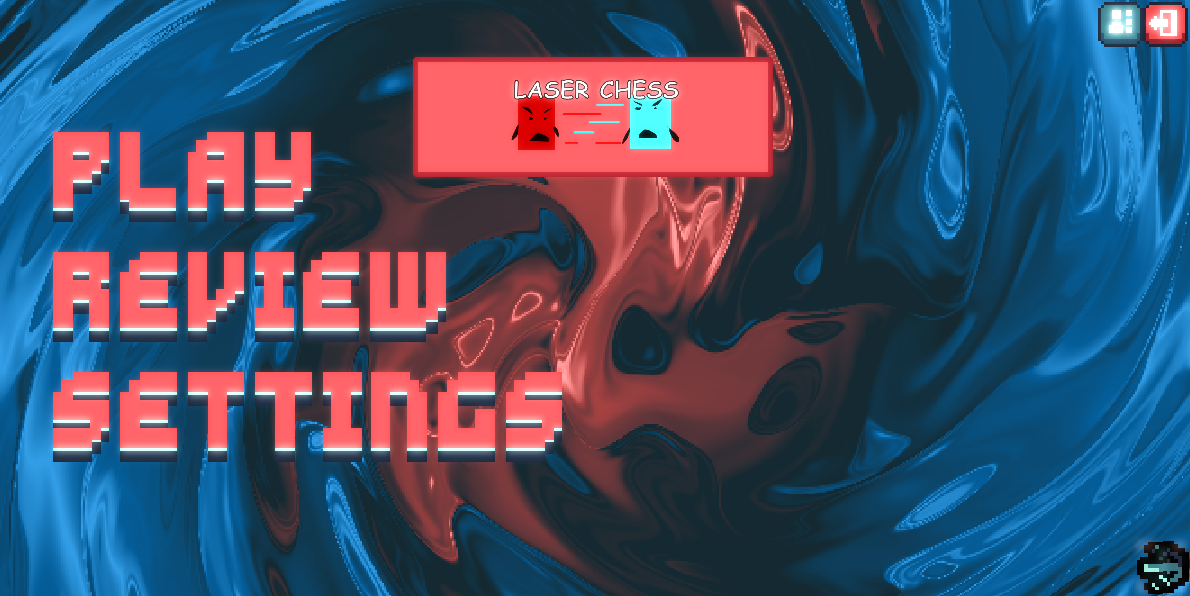
\includegraphics[width=\columnwidth]{../evaluation/assets/menu.png}
    \caption{Main menu screen}
    \label{fig:evaluation-menu}
\end{figure}

\begin{figure}[H]
    \centering
    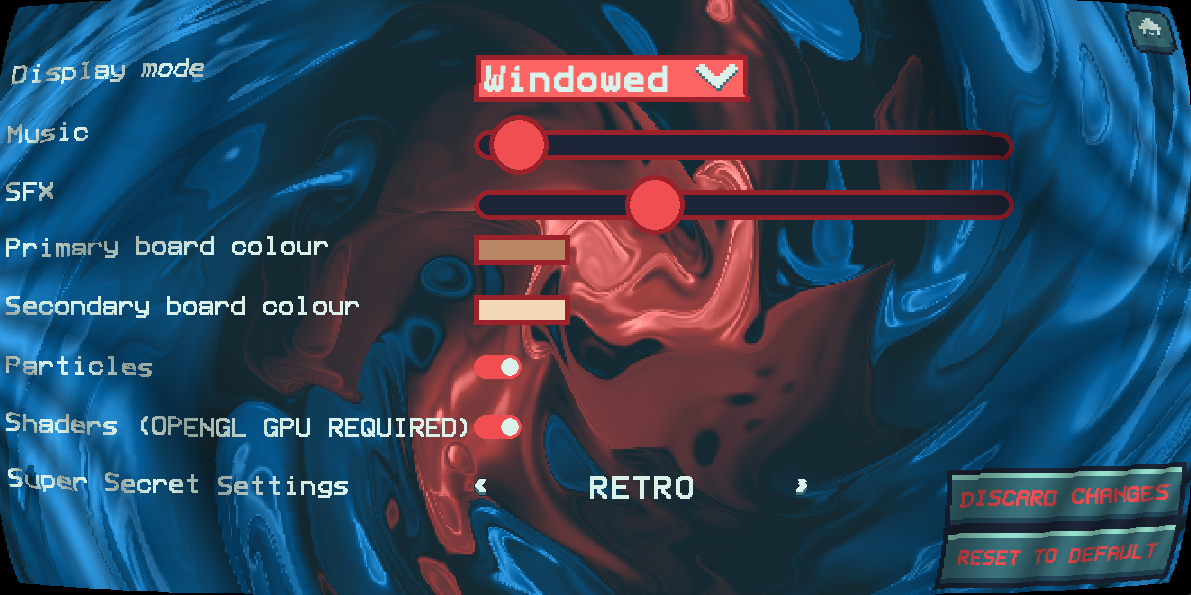
\includegraphics[width=\columnwidth]{../evaluation/assets/settings.png}
    \caption{Settings screen}
    \label{fig:evaluation-settings}
\end{figure}

\begin{figure}[H]
    \centering
    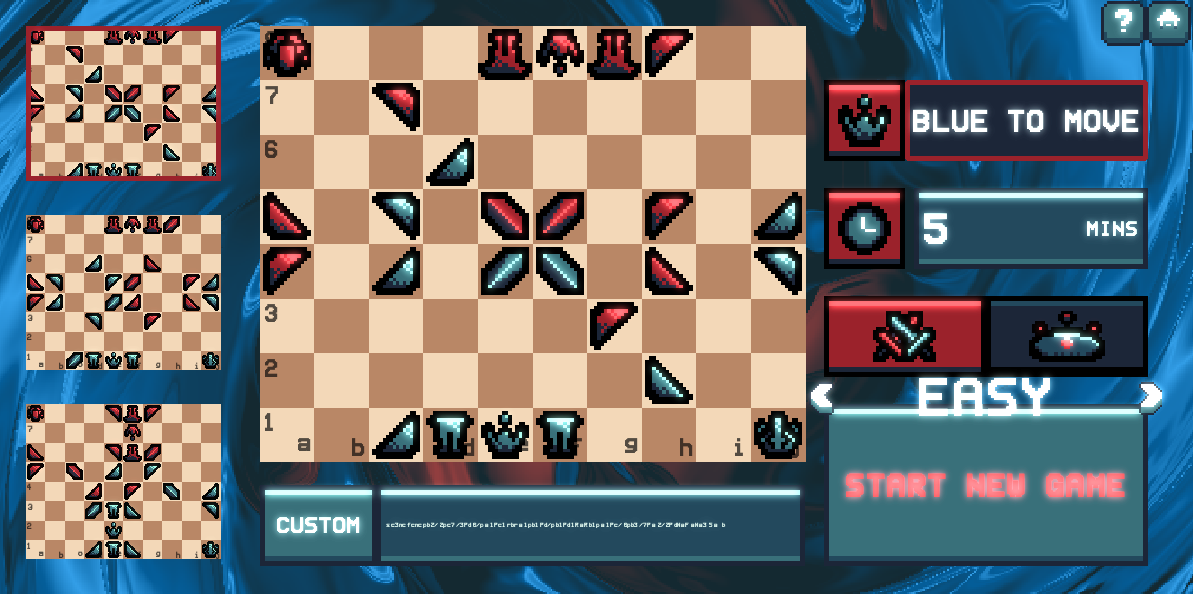
\includegraphics[width=\columnwidth]{../evaluation/assets/config.png}
    \caption{Config screen}
    \label{fig:evaluation-config}
\end{figure}

\begin{figure}[H]
    \centering
    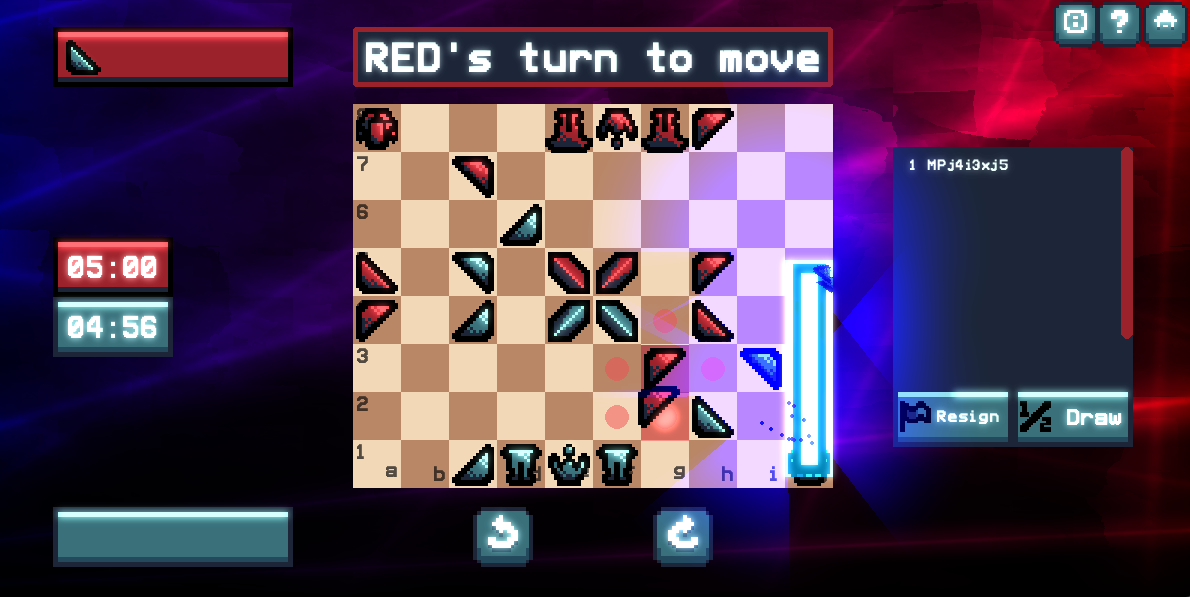
\includegraphics[width=\columnwidth]{../evaluation/assets/game.png}
    \caption{Game screen}
    \label{fig:evaluation-game}
\end{figure}

\begin{figure}[H]
    \centering
    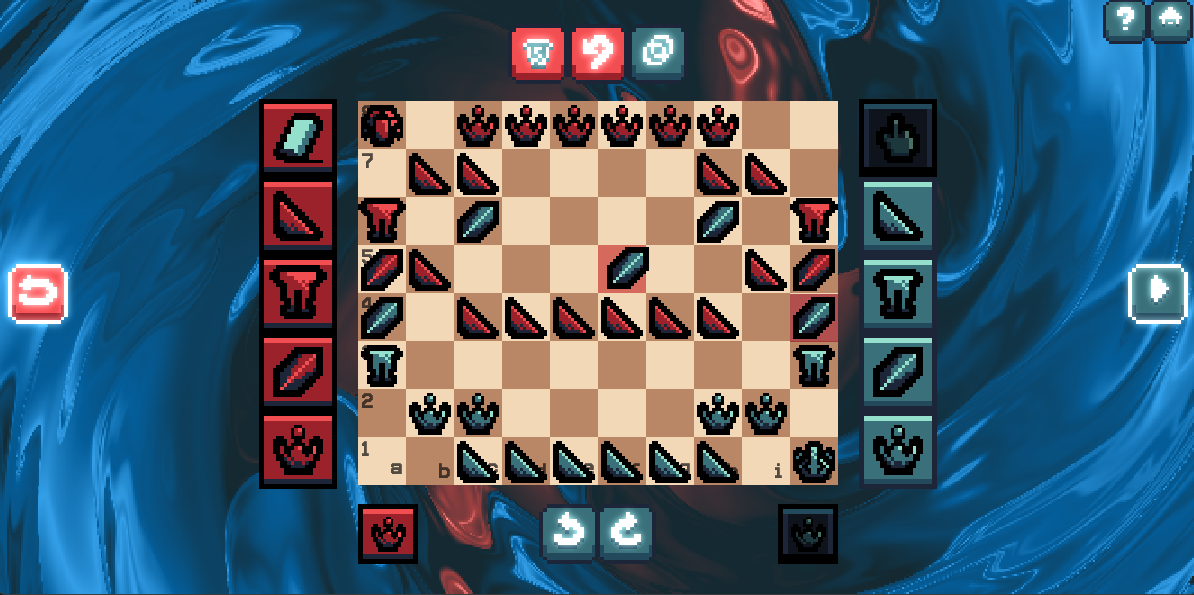
\includegraphics[width=\columnwidth]{../evaluation/assets/editor.png}
    \caption{Editor screen}
    \label{fig:evaluation-editor}
\end{figure}

\begin{figure}[H]
    \centering
    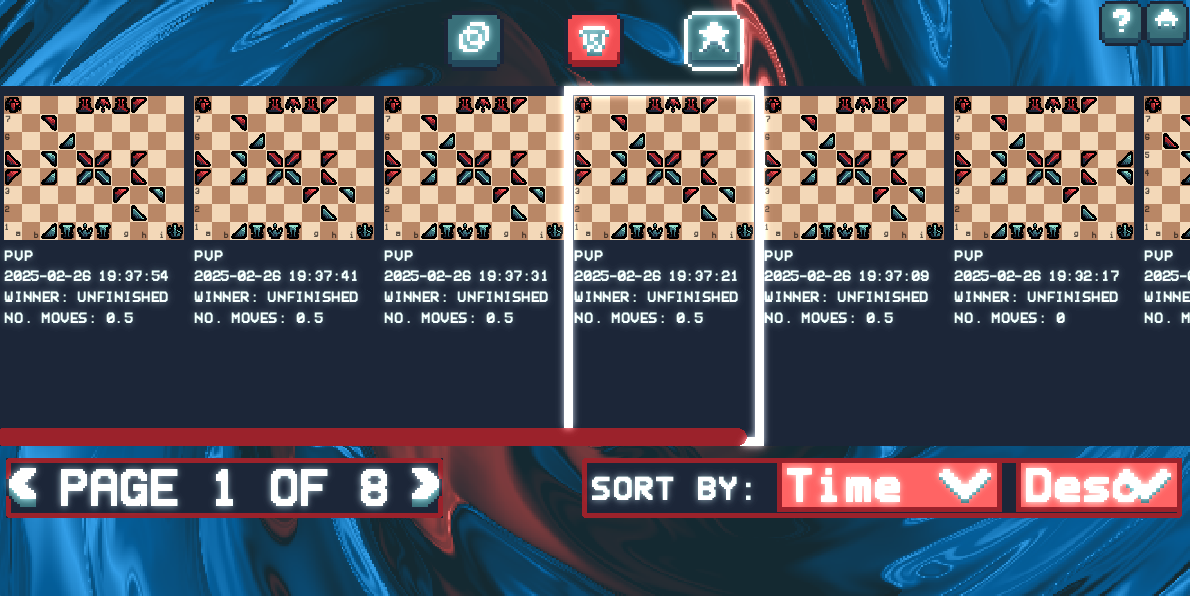
\includegraphics[width=\columnwidth]{../evaluation/assets/browser.png}
    \caption{Browser screen}
    \label{fig:evaluation-browser}
\end{figure}

\begin{figure}[H]
    \centering
    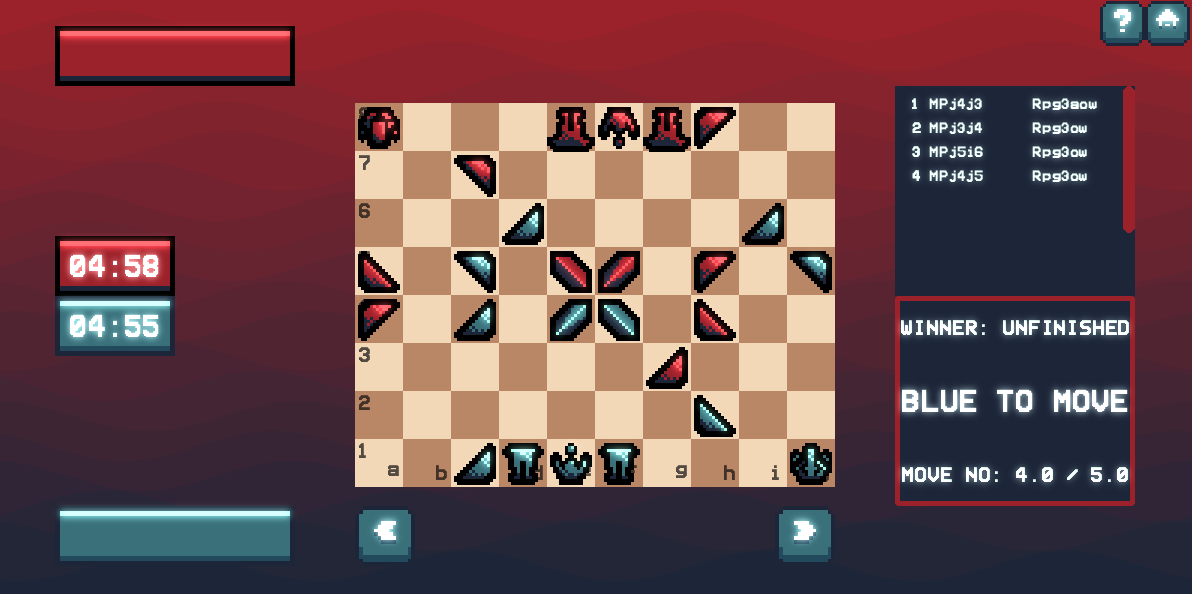
\includegraphics[width=\columnwidth]{../evaluation/assets/review.png}
    \caption{Review screen}
    \label{fig:evaluation-review}
\end{figure}

\end{document}